\chapter{Stanovení požadavků systému}

Cílem tohoto projektu je návr, realizace a otestování gatewaye, která shromažďuje data z bezdrátových koncových zařízení a přeposílá je přes RS485 LAN na PC master, který je dále přeposílá na IMA K4 server, kde jsou data zpracovávány.
\\
Předpokládá se, že koncová zařízení jsou senzory nebo aktuátory napájeny z baterie, tudíž pro jejich dlouhodobou životnost je kladen důraz na nízkou spotřebu vybrané bezdrátové technologie.
\\
Drátová síť RS485, přes kterou gateway komunikuje se PC masterem používá síťový protokol původně navržen pro přístupové systémy. 

\begin{figure}[!h]
    \centering
    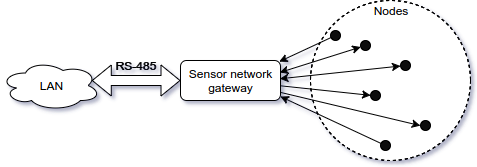
\includegraphics[width=1\textwidth]{01}
    \caption{Blokový diagram navrženého systému}
    \label{fig:block diagram of the system}
\end{figure}
